\documentclass[a4paper, 18pt]{article} % A4 paper, readable font size
\usepackage{geometry} % Adjust margins
\geometry{top=0.8in, bottom=0.8in, left=0.8in, right=0.6in} 


% packages we'll need...

% for controlling page numbers
\usepackage{fancyhdr}
\pagestyle{fancy}
\fancyhf{}
\fancyhead[R]{\thepage}

% throw in page-top header
\fancyhead[L]{Applying \textbf{TRANSFORMATICS} in GENETICS}

% for graphics
\usepackage{graphicx}
\usepackage{caption}
\usepackage{float}

% for drawing text boxes

% for proper treatment of urls
\usepackage{hyperref}

% for tables
\usepackage{tabularx}

% for line-breaks in table cells
%\usepackage{makecell}

% for long tables
\usepackage{longtable}
% for custom table col widths
\usepackage{array}
\newcolumntype{L}{>{\centering\arraybackslash}m{2cm}}
\newcolumntype{M}{>{\centering\arraybackslash}m{5cm}}

% for json listings...
\usepackage{listings}
%\usepackage{minted}
%\usemintedstyle{xcode}% no parser errors in listings?
%\usemintedstyle{bw} % grayscale color in listings, but shows parser errors!

% for maths
\usepackage{amsmath}
% for number sets symbols
\usepackage{amssymb}
%\usepackage{ntheorem}
\usepackage{amsthm}

% extra symbols
\usepackage{textgreek}
%\usepackage{mnsymbol}

% for writing our theorems and defs...
\newtheorem{comp}{Computation}
\newtheorem{theo}{Theorem}
\newtheorem{defn}{Definition}
\newtheorem{lem}{Lemma}
\newtheorem{prop}{Proposition}
\newtheorem{axiom}{Axiom}
\newtheorem{post}{Postulate}
\newtheorem{trans}{Transformation}
\newtheorem{transf}{Transformer}
\newtheorem{law}{Law}

% for highlighting text
\usepackage{xcolor, soul}
\definecolor{highcolor}{rgb}{0,255,255} %a color for background, that is friendly on black text foreground
\sethlcolor{highcolor}


% for wrapping text around floats
\usepackage{wrapfig}

% to include pdf pages
\usepackage{pdfpages}

% for multiline comments...
\newcommand{\comment}[1]{}

% for the cardinality symbol
\newcommand{\invpi}{\rotatebox[origin=c]{180}{$\pi$}}

\title{Applying \textbf{TRANSFORMATICS} in GENETICS}


\author{Willrich J. Lutalo\thanks{Currently a volunteering \& Independent Researcher at Nuchwezi Research --- \url{https://nuchwezi.com}}\\
\texttt{joewillrich@gmail.com, jwl@nuchwezi.com}}


\begin{document}

% insert [front] cover --- could just be a PNG or PDF
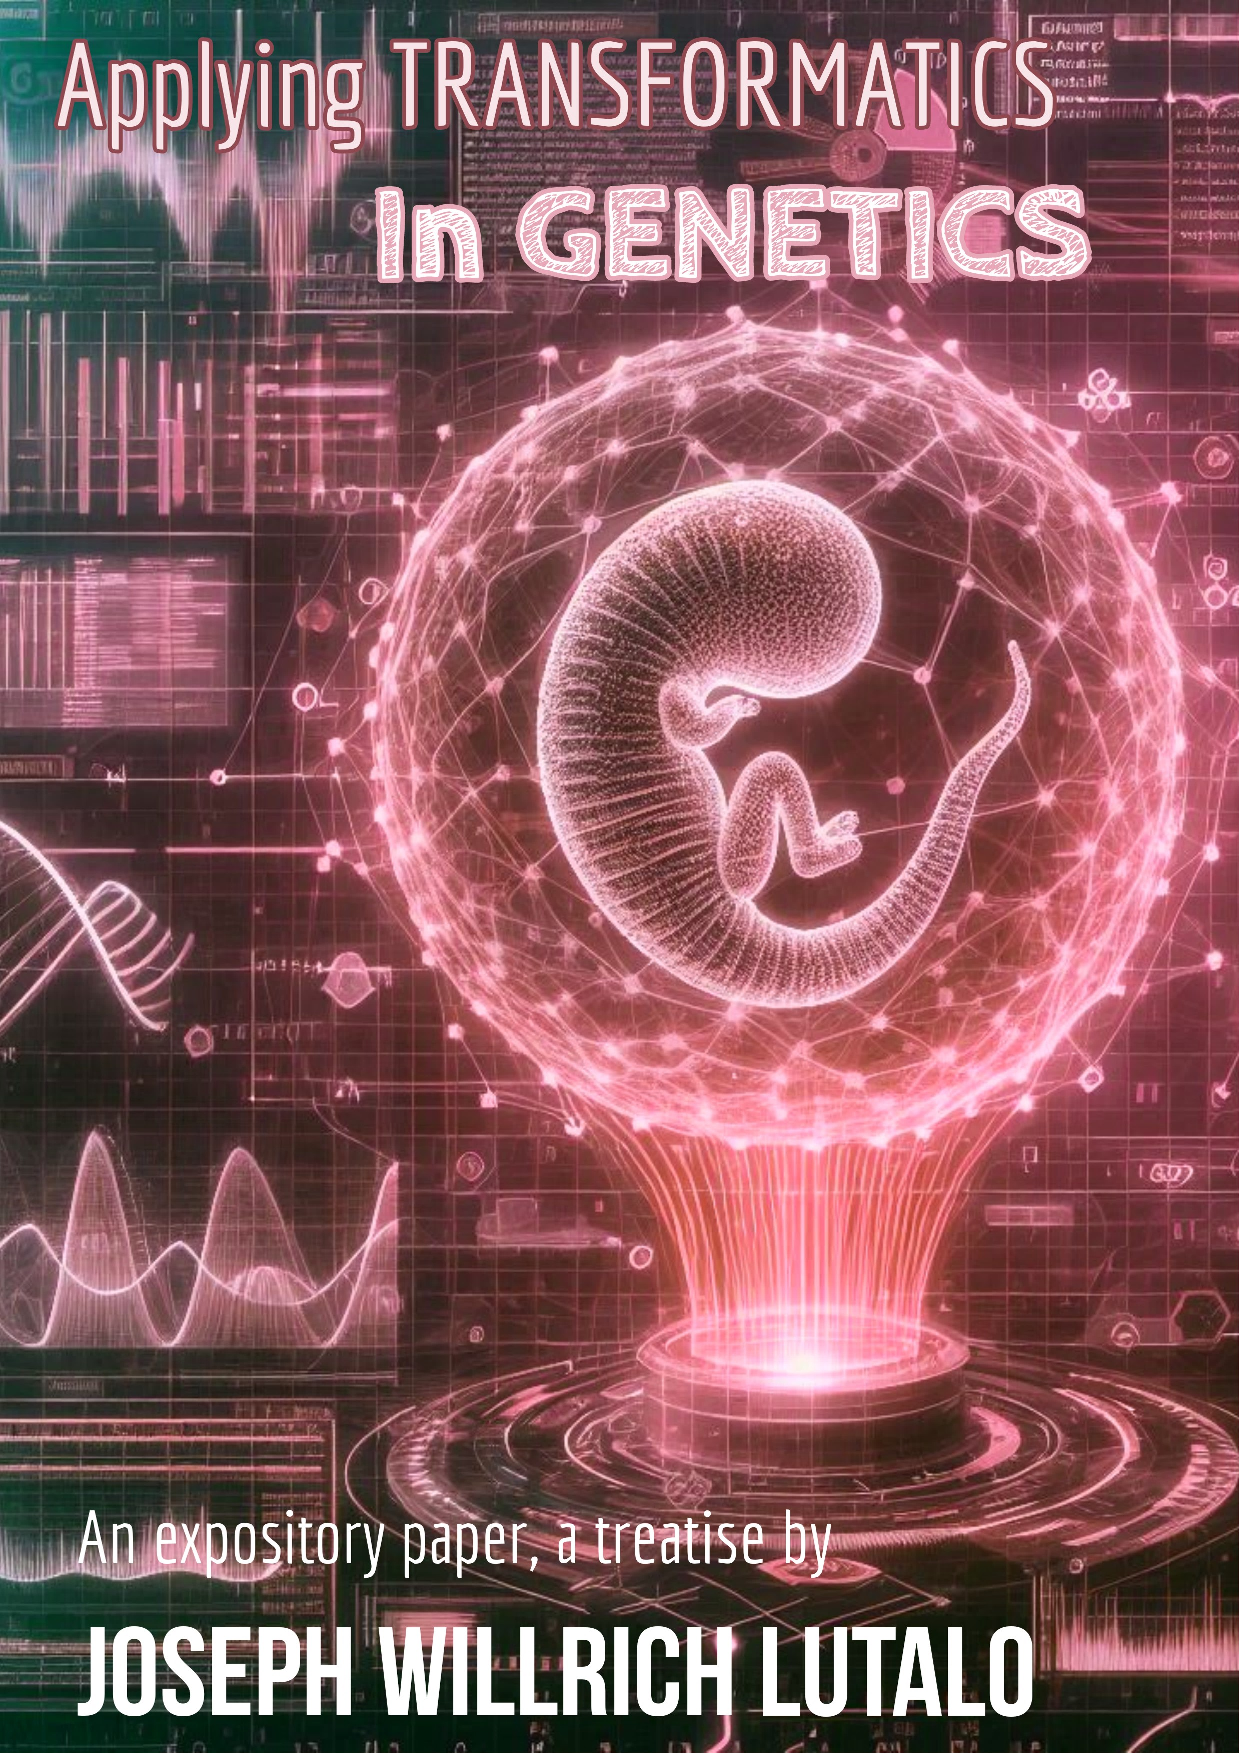
\includepdf[pages=1]{resources/pdfs/front_cover.pdf}

\maketitle


\Large

\begin{abstract}
\large

Though still just a paper, this work brings to surface the importance of leveraging the mathematical statistical theory recently named ``Transformatics", that deals with the study, processing and analysis of especially ordered sequences of symbols. It has been demonstrated to be a credible theory in designing, specifying or explaining the properties of automata operating on sequences to produce other sequences --- so-called sequence transformers. So, in this particular work, we take that body of knowledge, as well as what we know about the critically important science of how biological life-forms get to be defined, transformed and expressed in nature via the special genetic code known as DNA (deoxyribonucleic acid), that is best modeled conceptually as an ordered sequence of genes or more technically, a sequence of special combinations of any of four chemical bases (amino acids) or just ``nucleobases" --- Adenine(A), Cytosine(C), Guanine(G), and Thymine(T), into a finite sequence typically expressed as a double-helix ladder structure, that can then be decoded by convenient biological mechanisms so as to express or rather, manufacture one or more essential life-building compounds such as proteins that underlie the synthesis of specialized aspects of the organism's body such as skin, bone and muscle tissue in an animals or into cell-wall tissue, photosynthesis machinery and others, for plant organisms. This work demonstrates how several ideas first compiled under the transformatics umbrella can be well applied in problems relating to general genetics; we for example see how to quantify how far apart or different any two organisms might be based on the anagram distance between their genetic codes, this likewise being applicable to also sub-sequences of DNA that might underlie the expression of  just particular biological machines or mechanisms. We also consider how to leverage the concept of the modal sequence statistic in analyzing not just how similar different DNA sequences might be in terms of their relative composition of the basic nucleobases, but also in terms of their relative composition at higher abstraction levels such as at the level of amino-acids or large n-gram subsequences. We finally consider the matter of how, by leveraging the idea that a modal sequence encodes a summary about some larger sequence or an entire population of them, that we can then approach DNA as though it were a special statistical summary just like the MSS from transformatics theory, and then like how complex sequences could be constructed from summary statistics via certain protraction and multiplication transformers in earlier work, we use a thought experiment to demonstrate how DNA would be transcribed into both an mRNA-like structure and then which can be further transcribed into actual body structures that allow the organism to occupy space and appear or behave in a particular way. Though this work is mostly theoretical, we anticipate that this discussion and exposition shall inspire actual domain experts and other researchers interested in genetics, genetic engineering and other sciences to pick up and apply our transformatics theory and ideas in both theory and practice.
     \newline\newline
     \textbf{Keywords}: Applied Mathematical Statistics, Transformatics, Artificial Statistical Intelligence, Information Processing, Ordered Sequences, DNA sequences, Genetic Code, Genetic Analysis
\end{abstract}

\begin{quotation}
\noindent \texttt{Sex seems to have been invented around two billion years ago. Before then, new varieties of organisms could arise only from the accumulation of random mutations --- the selection of changes, letter by letter, in the genetic instructions. Evolution must have been agonizingly slow. With the invention of sex, two organisms could exchange whole paragraphs, pages and books of their DNA code, producing new varieties ready for the sieve of selection. Organisms are selected to engage in sex --- the ones that find it uninteresting quickly become extinct. And this is true not only for the microbes of two billion years ago. We humans have a palpable devotion to exchanging segments of DNA today.}\\
\hspace*{\fill} --- \textbf{Carl Sagan}, \textit{COSMOS}, 1981\cite{sagan1981cosmos}
\end{quotation}



\section{Introduction}
\label{SEC1}


\begin{quotation}
\noindent \texttt{The material basis of heredity is DNA, a ladder-like molecule which carries a message in the form of a `four-letter' code, the letters being four chemical bases, each of which may occupy any rung in the ladder.}\\
\hspace*{\fill} --- \textbf{The Oxford Companion to the Mind}\cite{gregory1987oxford}
\end{quotation}


In reality, we find that living, real organisms are influenced by genetics, their environment, bits of randomness and sometimes emergent behaviors that might not be readily captured by strict rules such as the genetic code of life. However, away from all possibilities, and focusing on what can be said of life expression via the genetic code known as DNA (the \textit{deoxyribonucleic acid}) or RNA (ribonucleic acid), especially when applied to the vast spectrum of natural organisms on earth --- from basic \textbf{prokaryotes} (single-celled organisms) such as the simple bacteria that actually have no nucleus\cite{bioexplorer2025}, to  \textbf{eukaryotes}; all the way from basic one-cell kinds such as amoeba\cite{kang2017deep} all the way to sophisticated creatures such as oak trees, vultures, dolphins and human beings! Talking of which, it might be important to set clear that though \textbf{viruses} are a kind of life-form\cite{libretexts2025viruses}, and yet, they are neither prokaryotes nor eukaryotes --- especially because, fundamentally, they are merely some genetic code (DNA or RNA) ``enclosed in a protein coat, lacking cell membranes or organelles"\cite{libretexts2025viruses} --- more technically they are \textbf{acellular entities}.

So, if we bring on-board ideas from \textbf{transformatics}\cite{transformatics} --- a new mathematical statistics theory dealing with sequences of symbols or those of named structures and their processing as well as analysis, for example, if we take the concept of leveraging statistical measures to summarize essential properties of sequences such as DNA --- say, with use of the modal sequence statistic (MSS), we find that, independently of, and without needing to first consult or worry about mainstream genetic code analysis or genetic engineering theory and mechanics, that we can say many useful things about genetic code sequences and that we might be able to break new ground or solve some otherwise still intractable problems concerning sequences of genetic code.




For example, by borrowing a useful DNA-as-library metaphor from Venville et al\cite{venville2006analogies}, we would come to appreciate that by looking at \textit{DNA as a library of books}, we have a model such as:

\begin{enumerate}
\item \textbf{Library}: DNA (as a whole) --- the \textbf{Genome},	 as the complete collection of genomic data about an organism.
\item \textbf{Bookshelves}: \textbf{Chromosomes} as organized storage of genes, and that they (chromosomes) are long, coiled-up strands of pairs of genes (essentially, the chromosome is a combination of two strands of genes, with one called the \textit{template} and the other a \textit{complement}, and that when they come together to form the ``ladder" structure, at each step, the two genes forming a step are paired such that $A \leftrightarrow T$ and $C \leftrightarrow G$ \cite{passel_dna_structure} --- also see \textbf{Figure \ref{FIG1}}). So, for example, humans have 46 chromosomes in total in their ``DNA library" (23 chromosome pairs, consisting of 22 autosomal pairs plus one pair of sex chromosomes). We know that during reproduction, the [full] genome (46 chromosomes in humans) splits up by half in either parent (via \textit{meiosis}, which somewhat shuffles the complete genome and then halves it\cite{genomics2025origin}), so that only one-half of the otherwise well-paired template-complement set that is the chromosome strand from each parent (as either sperm or ovum) goes to contribute to the final chromosome collection-set of the offspring\cite{libretexts2025gametogenesis}\cite{gregory1987oxford}. Whereas, after fertilization or during normal cell division, the entire chromosome set (with well-paired strands) is duplicated/replicated wholesomely and losslessly so that the second/new cell thus created has an exact copy of the same chromosome set (entire genome) as was in the source cell\cite{leicester_cellcycle}. 
\item \textbf{Books}: The \textbf{Genes} which make up a chromosome are the books in our genome library. Each gene is essentially a collection of ``words" that are a sequence of one or more codons (see below), and which taken together, contain enough information/instructions to specify how to produce a specific protein\cite{gregory1987oxford}\cite{venville2006analogies}.
\item \textbf{Words}: And then, under genes, we have \textbf{Codons} that are like ``words" in each book, and each codon \textbf{only} codes for a single \textbf{amino acid}. Basically, a codon is a combination of any 3 of the ``letters" of genetic code, for which, there are exactly four for DNA (A, C, G, T) and four for RNA (A, C, G, U). We also know that there are at most, 64 possible unique combinations of the four letters into triplets/3-grams/the codons\cite{gregory1987oxford}.
\item \textbf{Letters}: Finally, at the most basic level of our genetic code/DNA-library/genome, we have ``letters" that are technically known as \textbf{nucleotides}, and the nucleotide essentially each contains \textbf{a single nucleobase}, with only one difference between DNA and RNA as such; for DNA: $\{A, C, G, T\}$, and for RNA: $\{A, C, G, U\}$ --- we have seen the names of the four letters for DNA, and the new one for RNA, `U', stands for ``Uracil".
\end{enumerate}


So, with that introduction clearing up much of the basic genetics nomenclature and concepts that we shall use in the rest of this work, we then dive into the meat of our undertaking as such; \textbf{Section \ref{SEC2}} shall introduce the use of terminology and notation from transformatics to describe facts about genome sequences at various levels of abstraction. We shall look at using sequence symbol sets, sequence abstraction using sub-sequence symbols that can later be re-transformed into flat sequences, the idea of sequence cardinality when applied to DNA sequences and more. Then in \textbf{Section \ref{SEC3}} we shall deepen our discussion by considering how some of the measures from transformatics might be applied in genetic sequence analysis. We shall look into the ADM and PCR especially --- the other for cases where any two sequences are of the same length and similar symbol sets, and the other for cases where these need not be the same across the sequences under analysis. Then in \textbf{Section \ref{SEC4}} we shall take on the interesting matter for how, despite being merely a sequence of symbols, genetic code sequences actually can be likened to how a MSS can be used to specify how to reconstruct some other sequence. First, in \textbf{Section \ref{SEC05}} we shall first look at an overview of how actual interpretation or execution (more conventionally just referred to as ``gene translation") results in the manufacturing of proteins, and shall likewise look at some example actual gene translation in general and with a particular case. In \textbf{Section \ref{SEC5}} we shall then dive into a more hands-on exploration of this matter, with a hypothetical genome system (the \textbf{Numero-Gene Code}) that can allow us to not only creatively explore what genetic code is about, but which can also allow us to approach the rather complex matter of how DNA gets interpreted/translated into actual living tissue as well as a complete living organism. We shall introduce some two systems for how to decode our numero-gene DNA code into a kind of mRNA via the \textbf{Ozin-Transformer} and from ozin-gene code into actual tissue/proteins via the \textbf{Plato-Form Generator} that allows us to transcribe DNA into an orgnanism that has a predictable characteristic appearance and geometry, but also which still contains its essential genetic code just like normal living organisms do. Then we shall wrap-up in \textbf{Section \ref{CONC}}, looking at what we have accomplished, what remains to be done, and what the implications of this undertaking might be.

\section{Sequence Symbol Sets and Sequence Transforms Applied to Genetic Code}
\label{SEC2}

For the purposes of appreciating transformatics from a genetics engineering or general genetics research perspective, it shall be important to note that like in the original transformatics paper\cite{transformatics}, beginning by appreciating that whatever formalisms and mechanics we might develop or talk about concerning genetic code or rather DNA, had better begin with an appreciation that we can model DNA as merely an ordered sequence of symbols.

In the introduction (see \textbf{Section \ref{SEC1}}), we have already called out both the names and symbols assigned to the most basic units of any genetic code; essentially, the \textit{nucleobases} (or rather, nucleotides). For purposes of simplifying our mathematical logic later on, we shall here neatly define what roles these units play in the grand scheme concerning DNA and RNA code. Basically, we shall want to define the symbol sets for any DNA sequence and the symbol set for any RNA sequence.\\

\fbox{\begin{minipage}{0.9\textwidth}
\large

\begin{defn}[The \textbf{DNA Symbol Set}, $\psi_{DNA}$]
\label{DEFDNASS}

For any possible sequence of standard \textit{deoxyribonucleic acid} (\textbf{DNA}) for any possible living organism, the distinct nucleic acid base units are known as nucleotides\cite{wikipedia_nucleic_acid}, and these are essentially and exactly only four\footnote{Actually, or rather, in general, for nucleic acid sequences, the bases are four for either DNA or RNA, but, there are also conventions that extend this set to 17 or more to cater for cases like where there might be ambiguity about what the exact nucleotide in a particular position might be\cite{wikipedia_nucleic_acid}.};
\begin{itemize}
\item Adenine(A)
\item Cytosine(C)
\item Guanine(G)
\item Thymine(T)
\end{itemize}
And these are mapped to their representative, distinct single-letter symbols as shown. Thus, any possible DNA sequence must always consist of only one or more of those elements and nothing else. Thus, we might sum this up, using the symbol set concept\cite{Lutalo2024gtnc} as applied to sequences\cite{transformatics} as such:

\begin{equation}
\label{EQSSDNA}
\psi(DNA) = \{A, T, C, G\}
\end{equation}

\textbf{Equation \ref{EQSSDNA}} helps to appreciate the extra non-intuitive fact that the special ordering of DNA base symbols in the order A-T-C-G is what is conventionally accepted\cite{nature_atcg}\cite{wikipedia_nucleic_acid} or commonly found in most genetics literature\footnote{It shall be important to bring it out at this point, that, especially for non-domain experts --- people not trained in or normally practicing in genetics or related fields, that the common ordering of the nucleotides in the A-T-C-G ordering might seem unconventional or peculiar! For example, one might wonder, why are they not listed in their alphabetical order? So, for purposes of settings things clear for everyone, the author consulted a reliable research assistant on this matter\cite{copilot_dna_assistant}, and it was made clear that: ``The order **A, T, C, G** isn't alphabetical, and yet it's the most commonly used sequence when referring to DNA bases." We further learn that, the order A-T-G-C reflects a mix of historical usage and bio-chemical structure; \textbf{base-pairing logic}: that the DNA's double-helix is stabilized by ``complimentary base pairing" in which A pairs with T (via 2 hydrogen bonds), and C pairs with G (via 3 hydrogen bonds), so that listing A with its partner T and then C with G emphasizes this pairing symmetry\cite{copilot_dna_assistant}. Further, we learn that early molecular biology texts and sequencing protocols (especially post-Watson \& Crick, 1953) adopted this order to reflect the ``functional relationships" between bases. It became entrenched in educational materials, sequencing software, and databases. And lastly, that in visual and structural conventions --- such as in diagrams and models, A–T and C–G are often shown side-by-side. Listing them in this order reinforces the \textbf{duality} of the DNA ladder's rungs\cite{copilot_dna_assistant}. Lastly, that though there is no single documented moment when this convention begun, that the A-T-C-G order likely solidified in the \textbf{1970s - 1980s} during the rise of \textbf{Sanger sequencing} (developed in the 1970s), GenBank and EMBL databases, and overall in textbooks and molecular biology curricula.}.

However, and especially because, for transformatics, we wish to work with an \textbf{ordered symbol set}\cite{ossipaper} and not just \textit{any possible symbol set} so that we can apply mathematical logic that respects the ordering of terms in any ordered sequence\cite{transformatics}, we shall then assume a convention similar to how we might derive an ordered symbol set for a sequence of numbers in some base (the concept $\psi_\beta(\Theta)$ --- see \textbf{Definition 5} in \cite{ossipaper}), and given we are using Latin-Alphabet symbols (from $\psi_{az}$\cite{transformatics}) for $\psi_{DNA}$, we might as well better define the \textbf{Lexically Ordered DNA Symbol Set}, $\psi_{DNA}$ as such:

\begin{equation}
\label{EQDNASS}
\psi_{DNA} = \psi_{az}(DNA) = \langle A, C, G, T\rangle
\end{equation}

For all practical purposes unless where we merely wish to emphasize adherence to the tradition of ordering the nucleotides by their pairing order, we shall essentially imply $\psi_{az}(DNA)$ or rather $\psi_{DNA}$ when we talk of the \textbf{DNA Symbol Set}.

\end{defn}

\end{minipage}}
\\


Now that we have $\psi_{DNA}$ and $\psi_{RNA}$ well defined, we might immediately apply them to their finest use here: defining and supporting the special symbol set, $\psi_{na}$, that would or could allow for several kinds of nucleic acid sequences --- such as DNA for code stored in chromosomes and mitochondria, various kinds of RNA (\textit{m}RNA, \textit{t}RNA,...) and even synthetic/artificial/conceptual and also \textbf{random nucleic acid sequences}, etc. using a single universal nucleic acid symbol set. Thus we define $\psi_{na}$ below:


\begin{defn}[The \textit{\textbf{Universal Nucleic Acid Symbol Set}}, $\psi_{na}$]
\label{DEFUNA}
Any nucleic acid sequence, $\Theta$, obeys the following law:

\begin{law}[\textbf{Nucleic Acid Identifier Set}: $\psi_{na}$]
\label{LAWNA}
 The universal symbol set $\psi_{na}$ spans any nucleic acid sequence $\Theta$.
\begin{proof}
$\psi_{an} = \psi_{DNA} \cup \psi_{RNA} = \langle A, C, G, T, U \rangle$
\end{proof}
\end{law}
\end{defn}


As with many kinds of sequences dealt with in transformatics, the possession of a particular symbol set, such as $\psi_{na}$, allows for the practical use of those sets to implement logic systems that can operate on signal based on symbolic expressions of well ordered elements in sequences or sub-sequences. For this matter then, we shall likewise want to make formal, the concept of a \textbf{na-Sequence}:

\begin{defn}[The \textbf{$na-$Sequences} --- (D/R)-NA Sequences: $\Theta_{na}:\mathbb{N} \times \psi_{na}$]
\label{DEFNASEQ}

Any sequence of DNA or RNA nucleotides, expressible as some sequence of symbols from $\psi_{na}$ is a \textbf{na-Sequence} and its symbol set is a superset of both $\psi_{DNA}$ and $\psi_{RNA}$.

\end{defn}


If it is not immediately clear what the significance of \textbf{Defition \ref{DEFDNASS}} is or why it's important to unambiguously define $\psi_{DNA}$, then perhaps the mathematical discussions in later sections like \textbf{Section \ref{SEC3}} and \textbf{Section \ref{SEC4}} might this more obvious. That said, since we know that nucleic acid sequences come in two flavors\cite{wikipedia_nucleic_acid}, and since we have covered the essential ground for DNA symbol sets, we need now also consider the ordered RNA symbol set.\\


\fbox{\begin{minipage}{0.9\textwidth}
\large

\begin{defn}[The \textbf{RNA Symbol Set}, $\psi_{RNA}$]
\label{DEFRNASS}

For any possible sequence of standard \textit{ribonucleic acid} (\textbf{RNA}) for any possible living organism, the distinct nucleic acid base units are known as nucleotides\cite{wikipedia_nucleic_acid}, and these are essentially and exactly only four;
\begin{itemize}
\item Adenine(A)
\item Cytosine(C)
\item Guanine(G)
\item Uracil(U)
\end{itemize}
And these are mapped to their representative, distinct single-letter symbols as shown. Thus, any possible RNA sequence must always consist of only one or more of those elements and nothing else. Thus, we might sum this up, using the symbol set concept\cite{Lutalo2024gtnc} as applied to sequences\cite{transformatics} as such:

\begin{equation}
\label{EQSSRNA}
\psi(RNA) = \{A, U, C, G\}
\end{equation}

\textbf{Equation \ref{EQSSRNA}} helps to appreciate the traditional ordering of RNA base symbols in the order A-U-C-G reminiscent of the natural base-pairing order of DNA after it is translated into RNA (U merely replacing T)\cite{thoughtco_geneticcode}. And as with DNA, we shall want to have a proper, meaningful 
\textbf{ordered symbol set}\cite{ossipaper} for the RNA base symbols that we can later use in mathematical logic. Thus we shall equivalently define one for any standard RNA sequences as: 

\begin{equation}
\label{EQRNASS}
\psi_{RNA} = \psi_{az}(RNA) = \langle A, C, G, U\rangle
\end{equation}

And for all practical purposes in this work as well as after, we shall essentially imply $\psi_{az}(RNA)$ or rather $\psi_{RNA}$ when we talk of the \textbf{RNA Symbol Set} or the \textbf{Lexically Ordered RNA Symbol Set}.

\end{defn}

\end{minipage}}
\\


So, with those very essential definitions out of the way, we can begin to think of how we might appreciate and apply concepts from transformatics in genetics, in a clearer, straight forward manner.

For starters, we can certainly say that irrespective of how long or from where a particular DNA sequence, $\Theta_{DNA}$ originated from, once any sequence of data (e.g unstructured or unprocessed raw genetic code sequence dump), a string (say a proprietary encoding of some DNA code), a name (say of a particular species of interest and whose actual/representative genome sequence is know) or even a number (an id of a genome sequence in some standard genome database, etc.) is mapped to standard DNA sequence code, we shall know that any such transformation or mapping obeys \textbf{Theorem \ref{THEODNA}}:

\begin{theo}[$\psi_{DNA}$ is the alphabet of any DNA sequence]
\label{THEODNA}
For any sequence of DNA, $\Theta_{DNA}$, produced from some or any other source $\Theta$, irrespective of whether that source is itself a DNA sequence or not, we know that such an encoding or mapping, if it results in a valid DNA sequence $\Theta_{DNA}$, obeys the following general transformation:\\

\begin{trans}
\label{TRANSmDNA}
$\Theta \rightarrow \Theta_{DNA};$\\
$\forall a_{i \in [1,\invpi(\Theta_{DNA})]} \in \Theta_{DNA} \quad \exists \rho \in \psi_{DNA}: a_i = \rho$
\end{trans}

\begin{proof}
Assume $\Theta_{DNA}$ contains some symbol $\alpha$ such that $\alpha \not\in \psi_{DNA}$, it would contradict \textbf{Definition \ref{DEFDNASS}} which clearly states the legitimate membership of any DNA sequence.
\end{proof}

\end{theo}


And definitely, the equivalent truth for RNA sequences would likewise follow from \textbf{Definition \ref{DEFRNASS}}. So, we can then correctly tell that a sequence such as $\Theta_{insulin}$, which is the genetic code sequence defined as:\\


\fbox{\begin{minipage}{0.9\textwidth}
\large
%\begin{equation}
%\label{EQINSULIN}
\begin{multline}
\label{EQINSULIN}
\Theta_{insulin} =  \texttt{ATGGCCCTGTGGATGCGCCTCCTGCCCCTGCTGGCGCTGCTGGCCCTCTGGGGACC}\\
\texttt{CCAGCCGCAGCCTTTGTGAACCAACACCTGTGCGGCTCACACCTGGTGGAAGCTCTCTAC}\\
\texttt{CTAGTGTGCGGGGAACGAGGCTTCTTCTACACACCCAAGACCCGCCGGGAGGCAGAGGAC}\\
\texttt{CTGCAGGTGGGGCAGGTGGAGCTGGGCGGGGGCCCTGGTGCAGGCAGCCTGCAGCCCTTG}\\
\texttt{GCCCTGGAGGGGTCCCTGCAGAAGCGTGGCATTGTGGAACAATGCTGTACCAGCATCTGC}\\
\texttt{TCCCTCTACCAGCTGGAGAACTACTGCAACTAG}
\end{multline}
%\end{equation}
\end{minipage}}
\\

And which sequence\footnote{$\Theta_{insulin}$ is the short coding DNA sequence (CDS) for the human \textbf{INS} gene --- the part that gets transcribed into mRNA and translated by ribosomes into the insulin protein\cite{copilot_dna_assistant}}, despite having been obtained from an authority --- the \textbf{Leiden Open Variation Database (LOVD)}, which is based on NCBI's RefSeq data\cite{RefSeq}, might need to be verified by hand or with a critical eye, and that's where a law such as \textbf{Theorem \ref{THEODNA}} would come in handy. Also, note that, unlike common sequence notations we might see in this work or that we have encountered before, we wrote $\Theta_{insulin}$ in a manner somewhat more convenient for the kind of verbose sequence that DNA code generally is. The notation --- without opening or closing brackets around the sequence terms and neither commas in them might be reminiscent of the \textit{String [Chart] Sequence} notation we developed recently (see \textbf{Transformation 15} in \cite{transformatics}).

We might for example start to wonder, how might we go about determining if some two DNA sequences, $\Theta_1$ and $\Theta_2$ are the same or perhaps if they share parts of each other, and by how much? We might wonder if they are the same sequence merely shuffled/anagrammatized --- since we saw that this can occur during natural processes such as meiosis\cite{genomics2025origin}. In case they are different, we might want to for example quantify the relative frequency of their distinct members, e.g mapping $\psi_{DNA}$ or $\psi_{RNA}$ to a sequence of relative frequencies, etc. These are all things we shall soon look into and know very well how to do or talk about, using genetics terms and the mathematical language and techniques from transformatics.

\subsection{Sequence Abstraction: From Flat-Structure Sequences to Higher-Level Sequences}

Especially for nucleic acid sequences, but also for any other kind of sequence $\Theta$, there might be legitimate situations in which looking at or dealing with the flat-structure sequence --- such as for the actually modest\footnote{`Modest' because, genomes and realistic genome sequences can typically span millions of genes or billions of nucleotides. We for example know that for a typical human cell's DNA there are $\approx$3.2 billion base pairs\cite{Venter2001}, and yet we know each base pair consists of two nucleotides, one for each strand of the double-helix (so that's $\approx$6.4 billion), plus a few more ($\approx$16,569 base pairs) from mitochondrial DNA\cite{Anderson1981}} $\Theta_{insulin}$, might be cumbersome. And so, we are going to briefly look at ways that we might re-write verbose flat-sequences in more terse or higher-level abstract ways so as to focus on details that the flat-structure perhaps doesn't clearly express. This for example is naturally relevant in nucleic acid sequences since they are for example useful in scenarios where their processing is done in n-tuples/n-grams --- such as with codons (nucleotide 3-grams) or as gene programs (self-contained sequences of codons), etc.

So, assuming we have some sequence of symbols $\Theta_1$ defined as such:

\begin{equation}
\label{EQSEQ1}
\Theta_1 = \langle a_1, a_2,...,a_n\rangle
\end{equation}

If we wish to re-write the same sequence such that every $k$ terms are grouped in the same subsequence, we can then re-write $\Theta_1$ differently as such:


\begin{equation}
\label{EQSEQ2}
\Theta_2 = \Theta_2(n,k) = \langle a_{11}, a_{22}, a_{33}, a_{4k}, a_{51}, a_{62},...,a_{(n-k+1)(1)},...,a_{(n-k+k-1)(k-1)},a_{(n-k+k)(k)}\rangle
\end{equation}

Of course, in \textbf{Equation \ref{EQSEQ2}} we have somewhat wanted to extrapolate well and illustrate what would happen in an informative case such as when $k = 4$ and $n$ is not only significantly larger than $k$, but is also its perfect multiple. Otherwise, we might more concisely write that same sequence as:



\begin{equation}
\label{EQSEQ3}
\Theta_2(n,k) = \langle \langle a_1, a_2, a_3, a_4 \rangle_1, \langle a_5, a_6,...,a_8 \rangle_2,... , \langle a_{(n-k+1)},...,a_{(n-k+k-1)},a_{(n-k+k)}\rangle_{\frac{n}{k}} \rangle
\end{equation}

So, this expression in \textbf{Equation \ref{EQSEQ3}} is our first proper appreciation of what higher-level sequences might be like when they are an abstraction of normal flat-structure sequences. We see for example here, that the $k=4$ \textbf{bundling-parameter} means, we shall process the original flat sequence $k$ items at a time, and so, each subsequence in $\Theta_2(n,4)$ then contains exactly (or at most) 4 items --- we are assuming 4 is a factor of n to keep things simple. And so, we expect that, in total, we should have $\frac{n}{k}$ subsequences after applying the bundling transform:

\begin{transf}[The \textbf{k-GRAM Generator}]
\label{TRANSFBUND}
$\Theta = \langle a_1, a_2,...,a_n\rangle \quad \xrightarrow{O_{bundle-k}(\cdot)} \quad \Theta^* \quad;$\\
$\Theta^* = \langle \langle a_1, a_2,..., a_k \rangle_1, \langle a_{k+1},...,a_{2k} \rangle_2,... , \langle a_{(n-k+1)},...,a_{(n-k+k-1)},a_{(n-k+k)}\rangle_{\frac{n}{k}} \rangle$\\
$\forall a_i \in \Theta \quad \exists a_{ij} \in \Theta^*: a_i = a_{ij} \quad \land \quad j \in [1,k]$\\
For some $n, k \in \mathbb{N}$, and that $\invpi(\Theta^*) = \frac{n}{k} = $ number of k-gram subsequences generated from $\Theta$. $\qed$
\end{transf}


Thus, we see that the sequence depicted in \textbf{Equation \ref{EQSEQ3}} with $k=4$ could as well be produced by the generator defined in \textbf{Transformer \ref{TRANSFBUND}}. But not just that, if we applied that transformer to the DNA sequence $\Theta_{insulin}$ first presented in \textbf{Section \ref{SEC2}} --- see \textbf{Equation \ref{EQINSULIN}}, we can then produce a proper standard codon/3-gram mapping of that DNA sequence that would look something like:\\


\fbox{\begin{minipage}{0.9\textwidth}
\large
%\begin{equation}
%\label{EQINSULIN}
\begin{multline}
\label{EQINSUL2}
\Theta_{insulin} \xrightarrow{O_{bundle-3}(\cdot)}  \langle \texttt{<ATG>,<GCC>,<CTG>,<TGG>,<ATG>,<CGC>,<CTC>,...,<ACC>}\\
\texttt{...,<TAC>,<TGC>,<AAC>,<TAG>} \rangle
\end{multline}
%\end{equation}
\end{minipage}}
\\

And the way we have bundled up the nucleotides in \textbf{Equation \ref{EQINSUL2}} is exactly how a natural sequence processor such as a Ribosome (see details in \textbf{Definition \ref{DEFRIBOSOME}}) would process it so as to produce say a corresponding protein.

Of course, though we might not delve into it here or at the moment, we know that by chaining several sequence transformers --- such that one operates on the output of the previous one to produce the next sequence (see \textbf{Transformer \ref{TRANS1}} as an example), we can arrive at even higher abstraction sequences that might render certain sequence processing programs easier to write, analyze or define. For example, we know that, much as a Ribosome Processor operates on a sequence of codons, and yet, any legitimate protein synthesis and genetic code sequence processing program will require some sort of necessary delimiters (such as the START and STOP codons --- refer to the Protein Synthesis Flow Chart in \textbf{Figure \ref{FIG3}}), and so that, we might (if we could), abstract away codons and instead generate from a flat-structure DNA or perhaps mRNA sequence, a higher-level n-gram sequence of genes or \textbf{gene-program sequences}.


\section{Genetic Sequence Analysis Using Transformatics}
\label{SEC3}

We now turn our attention to the matter of using ideas from transformatics to help analyze or understand genetic code sequences. For starters, we shall want to consider the matter of how to tell how far apart or dissimilar any two nucleic acid sequences might be. Of course, consequently, that would also translate into meaningful way to tell how far apart not just low-level genetic-creations such as tissue, cell-types, proteins, etc might be based on the genetic code that produces them, but also how different entire organisms (within the same species or not) might be.

Because we can learn much about an organism based on its characteristic genome, and since that can be mapped to a flat-structure sequence of symbols such as we have already encountered in earlier sections, it might start to make sense to leverage the similarity/distance measures we have already developed so as to apply them to quantifying the distance between say species. In an earlier paper\cite{adtpaper}, we have introduced and also demonstrated how a sequence-analysis measure called the \textbf{Anagram Distance Measure}, $\tilde{A}(\Theta,\Theta^*)$, might be used to quantify how far apart some two sequences $\Theta$ and $\Theta^*$, that for the simplest scenarios better be of the same length, can be compared based on their common membership and the relative lexical ordering of the members in either sequence.

In the simple analysis we shall use to illustrate or develop our concepts, we shall deal with hypothetical nucleic acid sequences mostly --- especially DNA sequences, and their lengths shall be kept short to keep our analyzes simple, but also, their membership --- in terms of nucleotides, might have nothing to do with actual/natural sequences. The concepts and ideas we shall develop though, should be readily applicable to any or most nucleic acid sequences if not any sequences in general.

First, assume we have the following three sequences:

\begin{enumerate}
\item $\Theta_1 = CATGGGACTGCC$
\item $\Theta_2 = ATAATAAGAGGGATCTGA$
\item $\Theta_3 = AUAGGGAGAAUC$
\end{enumerate}

We can start by attempting to answer the question: \textbf{Which of these sequences are DNA and which are RNA?}

So, to answer that question, we can start by reducing each of those sequences to their respective [ordered] sequence symbol sets. In fact, if we first relax the assumption that they are either DNA or RNA sequences, and merely look at them as though they were any kind of sequence (for which we don't know the base or base-symbol set), then we can merely use the definition of an \textbf{Unspecific Symbol Set of $\Theta$ in Any Base} --- see \textbf{Definition 4} in \cite{ossipaper}. The algorithm for how to do that is simple and is well presented in that definition --- we basically create another sequence, in which we insert each distinct symbol from $\Theta$ that we encounter while processing the sequence from Left-to-Right\footnote{Such that the leftmost term is the first to be processed.}. Thus, we might construct the relevant transformer for this as such:

\begin{transf}[\textbf{Sequence Unspecified Symbol Set Generator}]
\label{TRANSSSGEN}$ $\\
$\Theta \xrightarrow{O_{suss-gen}(\cdot)} \Theta^* \quad;\quad \invpi(\Theta^*) \leq \invpi(\Theta) \quad \land \quad \Theta^* = \hat{\psi}(\Theta)$
\end{transf}

And thus, applying that transformer to the three sequences we have, we shall obtain the following results:

\begin{trans}
$\Theta_1 \xrightarrow{O_{suss-gen}(\cdot)} \langle C, A, T, G \rangle$
\end{trans}

\begin{trans}
$\Theta_2 \xrightarrow{O_{suss-gen}(\cdot)} \langle A, T, G, C \rangle$
\end{trans}

\begin{trans}
$\Theta_3 \xrightarrow{O_{suss-gen}(\cdot)} \langle A, U, G, C \rangle$
\end{trans}

At this juncture, we can then closely inspect the resultant sequences --- each of them a kind of symbol set, and then judge which of $\psi_{DNA}$ or $\psi_{RNA}$ they are associated with. To proceed in a rigorous manner, we might also want to compute the \textbf{Natural Symbol Set of $\Theta$ in some Base-$\beta$} --- see \textbf{Definition 5} in \cite{ossipaper}. A suitable transformer to compute such a symbol-set (for which, unlike the unspecific symbol set, orders the terms in the resultant sequence by their natural order of occurrence in the base's ordered symbol set) would as as such:\\


\begin{transf}[\textbf{Sequence $\beta$-Natural Symbol Set Generator}]
\label{TRANSNSGEN}$ $\\
$\Theta \xrightarrow{O_{snss-gen-\beta}(\cdot)} \Theta^* \quad;\quad \invpi(\Theta^*) \leq \invpi(\Theta) \quad \land \quad \Theta^* = \psi_\beta(\Theta)$
\end{transf}

And, since we already have an idea what the symbol sets for each of the three sequences are --- from which we can guess and/or disqualify some candidate bases --- e.g, since $\hat{\psi}(\Theta_3) \setminus \psi_{DNA} = \{U\}$, then $\Theta_3$ can't be a DNA sequence. However, to complete our analysis, note that:


\begin{trans}
$\Theta_1 \xrightarrow{O_{snss-gen-DNA}(\cdot)} \langle A, C, G, T \rangle$
\end{trans}

\begin{trans}
$\Theta_2 \xrightarrow{O_{suss-gen}(\cdot)} \langle A, C, G, T \rangle$
\end{trans}

\begin{trans}
$\Theta_3 \xrightarrow{O_{suss-gen}(\cdot)} \langle A, C, G, U \rangle$
\end{trans}

So, we can safely conclude that:

\begin{enumerate}
\item Since $\psi_{DNA}(\Theta_1) = \psi_{DNA}$, then $\Theta_1$ is a DNA sequence.
\item Since $\psi_{DNA}(\Theta_2) = \psi_{DNA}$, then $\Theta_2$ is a DNA sequence.
\item Since $\psi_{RNA}(\Theta_3) = \psi_{RNA}$, then $\Theta_3$ is a RNA sequence.
\item Even if we forced it, note that $\psi_{RNA}(\Theta_1) = \langle A, C, G, T \rangle \neq \psi_{RNA}$, or rather that $\hat{\psi}(\Theta_1) \setminus \psi_{RNA} = \{T\}$ so $\Theta_1$ can't be an RNA sequence.
\end{enumerate} 

Talking of which, in case we had some variation of $\Theta_1$ that has no instances of T in it, such as the sequence $\Theta_4 = CAAGGGACAGCC$, then we shall find that:

\begin{trans}
$\Theta_4 \xrightarrow{O_{suss-gen}(\cdot)} \langle C, A, G \rangle$
\end{trans}

and that:

\begin{trans}
$\Theta_4 \xrightarrow{O_{snss-gen-DNA}(\cdot)} \langle A, C, G \rangle \subset \psi_{DNA}$
\end{trans}

But also that:

\begin{trans}
$\Theta_4 \xrightarrow{O_{snss-gen-RNA}(\cdot)} \langle A, C, G \rangle \subset \psi_{RNA}$
\end{trans}

And thus, we have the peculiar case in which a nucleic acid sequence can both be a legitimate DNA or RNA sequence! However, such a truly peculiar sequence it is! Because, given the START-codon symbol set, $\psi_{na-START}$, a sequence of all the ``start" kind codons whether of DNA or RNA type, is defined as such from all we currently know:

\begin{defn}[The \textbf{Nucleic Acid START-codons}]
\label{DEFSTARTCOD}
For any known organism, prokaryote or eukaryote, the only legitimate and known codons of the START-kind are any of the codons or START 3-grams in the unordered sequence $\psi_{na-START}$, the \textbf{nucleic acid START-codon symbol set}.\\

\begin{equation}
\label{EQNNASSS}
\psi_{na-START} = \{ATG,AUG,GTG,GUG,TTG,UUG\}
\end{equation}\\

So, that, if say a nucleic acid program for producing some protein via some gene program $\Theta_{na}$ were to be processed by an ideal ribosome (see \textbf{Definition \ref{DEFRIBOSOME}}), the ribosome would never produce anything --- or, equivalently, there is no guarantee that any protein would be produced no matter what or any instructions the gene program contains, as long as it doesn't contain any one of the members of $\psi_{na-START}$.
\end{defn} 

One interesting consequence of that definition is the following law:

\begin{law}[\textbf{Non-Coding Gene Programs}]
If any gene-program $\Theta_{na}$ is processed by a ribosome, and yet it has the property:\\

 $\psi_{DNA}(\Theta_na) \cap \psi_{na-START} = \emptyset \quad \lor \quad \psi_{RNA}(\Theta_na) \cap \psi_{na-START} = \emptyset$\\
 
It implies that $\Theta_{na}$ shall never be executed by the ribosome, and neither shall it ever result in any new protein or new amino-acid product within the containing cell system\footnote{Refer to ribosome definition for details: \textbf{Definition \ref{DEFRIBOSOME}}}.
\end{law}


So, that, if say a nucleic acid program for producing some protein via some gene program $\Theta_{na}$ were to be processed by an ideal ribosome processor (see \textbf{Definition \ref{DEFRIBOSOME}}), the ribosome would never return --- or, equivalently, there is no guarantee that any products --- neither amino-acid, nor completed/new protein, shall be synthesized by the ribosome.

Of course, it's very likely that such gene sequences exist, and there might be nothing wrong with them being natural too. However, we shall want to learn more about this from the domain experts in the future.

That said, another, closely related case is that of the consequences of the STOP-codons or rather, the STOP-codon symbol set, $\psi_{na-STOP}$ defined as such:


\begin{defn}[The \textbf{Nucleic Acid STOP-codons}]
\label{DEFSTOPCOD}
For any known organism, prokaryote or eukaryote, the only legitimate and known codons of the STOP-kind are any of the codons or STOP 3-grams in the unordered sequence $\psi_{na-STOP}$, the \textbf{nucleic acid STOP-codon symbol set}.\\

\begin{equation}
\label{EQNNASSSTOP}
\psi_{na-STOP} = \{TAA,UAA,TAG,UAG,TGA,UGA\}
\end{equation}\\
\end{defn} 

Among important consequences of \textbf{Definition \ref{DEFSTOPCOD}}, is that, if say a nucleic acid program for producing some protein via some gene program $\Theta_{na}$ were to ever be processed by an ideal ribosome (see \textbf{Definition \ref{DEFRIBOSOME}}), the ribosome might produce something --- some amino-acids for example, but would never return --- equivalently, there is no guarantee that any protein would be released by the protein manufacturing process/ribosome, no matter what or how many any amino-acid productions and translate instructions the gene program contains and which have been executed by the ribosome. As long as the gene-program doesn't contain any one of the members of $\psi_{na-STOP}$ that is.

It is not immediately clear what the plausibility of such an \textit{evil gene-program} existing out there in nature might be, but given normal genes sometimes mutate\cite{gregory1987oxford}, it can't be ruled out that such awkward programs might exist. Though we won't dive into that here, who knows... from a computer security perspective, such a program might cause system errors or faults such as a System-Out-Of-Resources problem given the ribosome might attempt to produce an infinite length amino-acid, or perhaps that the cell's protein manufacturing closure might run out of space, or that the processor might end up hanging since the factory never is able to reach any of WAIT, DETACH or RESET states --- see \textbf{The Ribosome State Machine} in \textbf{Figure \ref{FIG4}} but also refer to the Protein Synthesis Process in \textbf{Figure \ref{FIG3}} to clearly, logically appreciate these kinds of problems and/or corner-case scenarios. 

That said, in case a normally correct gene-program such as what we saw in $\psi_{insulin}$ (see \textbf{Equation \ref{EQINSULIN}}) is altered with --- perhaps by a natural mutation, or perhaps a virus, or even in a totally malicious feat of gene-manipulation medicine, and such a transformation results in a nucleic-acid sequence satisfying any of the above queer cases, who knows, but it might as well be the root case of some difficult flaw in the organism --- an incurable and fatal disease (if the faulty gene-program is crucial for normal life support and that it has no alternatives or simple way to be solved), and these might the kinds of hard problems that might require not just medical doctors, biologists or perhaps genetists to tackle, but also people like computer hackers, information-security experts and software debuggers\footnote{It shouldn't come as a surprise, that with a stronger marriage of computing theory and biology, or medicine, that certain problems in nature --- not just with humans or animals, but also with plants for example, and especially if they are either inheritable --- meaning genetic, or if they might somehow be remedied via clever hacking or debugging and modifying of the organism via gene programs, might call for the skills of and expertise of software engineers and program debuggers from hardcore computer science and not just the medical or biological sciences! A great background work on this subject by the author might come in handy --- refer to \cite{Lutalo2025debug}}!


\section{The Modal Sequence Statistic as a Generic Genetic Code --- A Case of Bio-Automata}
\label{SEC4}

We are going to talk about the matter of the \textbf{Genetic Anagram Distance}, $0 \geq \tilde{A}(\Theta_{na} \rightarrow \Theta_{na}^*) \leq \infty$, between any two of species, populations, individual organisms or any entity specifiable via sequences. We are to deal with nucleic acid sequences mostly. 

Such a concept, derived from the ADM theory, can allow us to quantity by how much and/or if there is any significant variation between any two organisms, species or just arbitrary DNA sequences, given not just the composition of the DNA sequences themselves, but also the ordering of members within it matters in the mathematics and logic of processing, analyzing and or specifying \textbf{nucleic acid sequences} --- in which, as per . The following three hypothetical, but semantically and syntactically legitimate expressions of either DNA or mRNA nucleic acid sequences in formal sequence expressions:\\

\begin{equation}
{\Theta1}_{DNA} = \langle TAC GGG CAT TCC \rangle\\
\end{equation}

\begin{equation}
{\Theta2}_{RNA} = \langle AUG AUG CGC GGG CAU AUC \rangle\\
\end{equation}


\begin{equation}
{\Theta3}_{DNA} = \langle ATA ATGG GGG CAT TGA \rangle\\
\end{equation}





\section{Gene Expression in Living Organisms Leveraging Genetic Code (DNA $\rightarrow mRNA \rightarrow Protein \rightarrow$ Organism)}
\label{SEC05}


\begin{quotation}
\noindent \texttt{Code: A rule for transforming a message from one symbolic form (the source alphabet) into another (the target alphabet), usually without loss of information. The process of transformation is called encoding and its converse is called decoding.}\\
\hspace*{\fill} --- \textbf{The Oxford Companion to the Mind}\cite{gregory1987oxford}
\end{quotation}



\begin{figure}[H]
	\begin{center}
		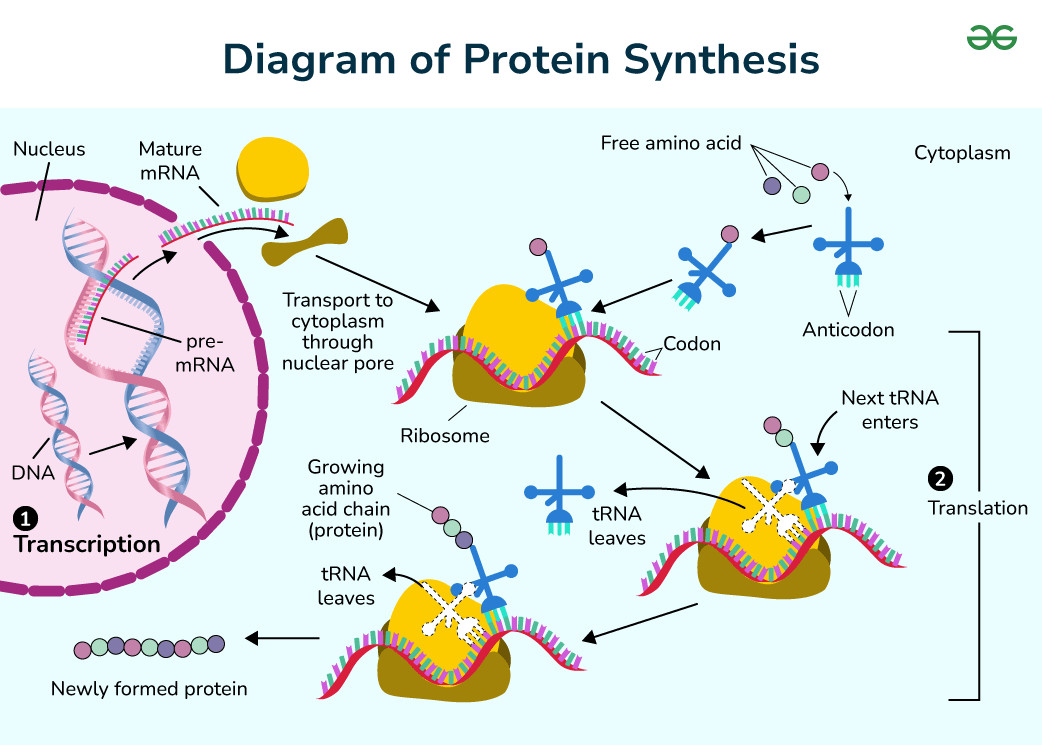
\includegraphics[width=0.9\textwidth]{resources/images/protein_synthesis.png} \\
		\caption{An illustration of the gene translation process in a cell via protein-factories known as ribosomes\cite{geeksforgeeks2024protein}}
		\label{FIG2}
\end{center}
\end{figure}
    
    
It shall be interesting to note that for genetic code in natural automata (nature-like bio-automata\footnote{My research assistant --- thanks \textbf{Microsoft Copilot}, did bring it to my attention that the term ``bio-automata" is ``usually reserved for models or conceptual representations of biological systems --- especially those designed to simulate behaviors, growth patterns, or decisions-making processes using predefined rules, like in cellular automata or agent-based modeling." And thus, much as I often find it attractive to use the term --- as an umbrella term including actual living organisms which, from the perspective of the computer scientist in me, are still correctly classifiable under the "biological automata" category in my opinion since they actually operate on some infallible inherent natural program in their DNA. But, I shall adhere to the advise of my assistant for now.} and generally living things), the most important reason the genetic coding language exists, is so that the body/host-organism system can produce required materials as and when they are needed or demanded for. This for example means producing new or extra body tissue in a still growing organism or in one with any damaged or missing tissue, and essentially, such productions are about the synthesis of particular molecules in the body's system that are basically proteins. The diagram in \textbf{Figure \ref{FIG2}} is a basic illustration of the process for living organisms --- eukaryotes especially.

For simplicity's sake, we can assume the following summarization of the basic process that fully and correctly breaks down the typical ordeal:

First, we shall assume that given the protein is just a chain of amino-acids, we might as well just think of it as though it were an ordered sequence of some terms, and thus, in keeping with the notation from transformatics, we might just refer to such a protein with our usual typical \textbf{resultant sequence} symbol --- $\Theta^*$.

And so, given that these proteins are actually nearly direct/1-to-1 mappings from the corresponding DNA sub-sequence code of a finite length, we might then refer to the DNA sequence that encodes the instructions for producing $\Theta^*$ with just the basic typical transformatics \textbf{source sequence} symbol: $\Theta$ --- more conveniently, because we wish to also talk of the length of the sequence, we might preferably write the DNA sequence code of length \textbf{n} (meaning for example, \textbf{it contains exactly n DNA-codons}), as $\Theta_n$. So, for example we might more fully express $\Theta_n$ as such:

\begin{equation}
\label{EQ1}
\Theta_n = \langle a_{ij}, \rangle ;
a_{ij} \in \psi_{DNA^*} \quad \forall j \in [1,n],  i \in [1,64] \quad \land \quad n \in \mathbb{N}
\end{equation}\\

\textbf{Equation \ref{EQ1}} being just a sometimes preferable way to write the same exact sequence as:
 
 
 \begin{equation}
\label{EQ2}
\Theta_n = \langle a_1,a_2,a_3,...,a_i,...,a_{n-1},a_n \rangle ;
\forall i \quad \exists a_i \in \psi_{DNA^*} \quad \land \quad n \in \mathbb{N}
\end{equation}\\

We have defined the special symbol sets $\psi_{DNA^*}$ in \textbf{Section \ref{SEC..}} and  $\psi_{DNA}$ in \textbf{Definition \ref{DEFDNASS}}, and as for $\psi_{DNA^*}$, we know that it essentially is the set of the distinct 64 codons (see \textbf{Table 1} in \cite{gregory1987oxford}) that \textit{especially} encode amino acids, and which were first introduced in \textbf{Section \ref{SEC1}}. Another way to expound on this is by saying that:

 \begin{equation}
\label{EQ3}
\Theta_n = \{a_i \quad | \quad a_i = \prod\limits_{\rho \in \psi_{DNA}}^3 \rho \quad \land \quad \forall i \in [1,n], n \in \mathbb{N} \quad \land \quad \psi_{DNA} = \langle A, C, G, T \rangle\}
\end{equation}\\

Thus we might encounter a gene such as $\Theta_4$ composed of exactly 4 codons as shown below:

 \begin{equation}
\label{EQ4}
\Theta_4 = \langle \langle A, T, G \rangle, \langle A, A, A \rangle, \langle T, T, A \rangle, \langle T, A, G \rangle \rangle
\end{equation}\\

Which, might also equivalently be expressed as a flattened sequence if the fact that the nucleobases it contains are always read in triplets/3-grams/tuples of 3 at a time. So that we can merely write it as:\\

 \begin{equation}
\label{EQ5}
\Theta_{4 \times 3} = \langle  A, T, G, A, A, A, T, T, A, T, A, G \rangle
\end{equation}\\

So we imply that under the flat-structure notation, the sequence has exactly $4 \times 3$ elements. By this fact and the observation that the previous nested notation merely helps to group together each codon's members within a meaningful sub-sequence, and that the order is otherwise maintained in the flat-sequence structure, we might then also equivalently express the same actual DNA code sequence as an $n \times 3$ matrix as shown below:

 \begin{equation}
\label{EQ5a}
\Theta_{4 \times 3} = \begin{pmatrix}
A& T& G\\
A& A& A\\
T& T& A\\
T& A & G \\
\end{pmatrix}
\end{equation}\\


Whether to actually express it as a $3 \times n$ matrix or as $n \times 3$ might be up to the particular taste of the mathematician or scientist, but otherwise, we know that the ordered sequence $\Theta$ in any of the forms above is essentially a \textbf{genetic program} to guide a DNA code processor such as a ribosome construct a corresponding protein based on the equivalent transcribed mRNA code sequence $\Theta_4^*$ written in mRNA code as such:


 \begin{equation}
\label{EQ6}
\Theta_4^* = \langle \langle A, U, G \rangle, \langle A, A, A \rangle, \langle U, U, A \rangle, \langle U, A, G \rangle \rangle
\end{equation}\\

Which is what we would obtain after a necessary \textbf{DNA} $\rightarrow$ \textbf{mRNA} transform attainable via a DNA sequence transformer we might define as such:\\


\begin{transf}[\textbf{DNA to mRNA Encoder}]
\label{TRANSF1}
$\Theta_n \quad \xrightarrow{O_{mRNA-encode}(\cdot)} \quad \Theta^*_n \quad;$\\
$\forall a_i \in \Theta_n = \langle a_i,\rangle:n, \quad a_i \in \psi_{DNA} \equiv \{A, T, C, G\}$,\\
and if $\exists a_i \in \Theta_n : a_i = T \implies \exists a_i^* \in \Theta^*_n: a_i^* = U$\\
Otherwise $a_i = a_i^* \implies \invpi(a_i = T \in \Theta_n) = \invpi(U \in \Theta^*_n) \quad \land \quad \invpi(\Theta_n) = \invpi(\Theta^*_n) = n$.

\end{transf}

\begin{table}[h]
  \centering
  \Large
	\begin{tabular}[t]{|c|c|c|p{3cm}|}
	\hline
	i & $a_i$ & \textbf{Amino Acid (Code-name)} & \textbf{Function}\\
	\hline
	\hline
	1 & ATG & Methionine (Met) & Start Codon: initiates translation\\
	\hline
	2 & AAA & Lysine (Lys) & Basic amino acid\\
	\hline
	3 & TTA & Leucine (Leu) & Non polar amino acid\\
	\hline
	4 & TAG & Stop (Amber) & Terminates translation\\
	
	\hline
	              
\end{tabular}
 \caption{Amino-Acid Codes and Names in $\Theta_4$, a DNA-encoded gene}
  \label{TAB1}
\end{table}

Thus, though the gene in its DNA form comprised of the ordered sequence of amino-acid codes named as in \textbf{Table \ref{TAB1}}, and yet, the resultant sequence after applying \textbf{Transformer \ref{TRANSF1}} to $\Theta_4$ would be as explained in \textbf{Table \ref{TAB2}}.


\begin{table}[h]
  \centering
  \Large
	\begin{tabular}[t]{|c|c|c|p{3cm}|}
	\hline
	i & $a_i$ & \textbf{Amino Acid (Code-name)} & \textbf{Function}\\
	\hline
	\hline
	1 & AUG & Methionine (Met) & Start Codon: initiates translation\\
	\hline
	2 & AAA & Lysine (Lys) & Basic amino acid\\
	\hline
	3 & UUA & Leucine (Leu) & Non polar amino acid\\
	\hline
	4 & UAG & Stop (Amber) & Terminates translation\\
	
	\hline
	              
\end{tabular}
 \caption{Amino-Acid Codes and Names in $\Theta_4^*$, a mRNA encoded gene}
  \label{TAB2}
\end{table}

So, note that the names (and code-names) of the mRNA encoded codons stay the same as those of their corresponding DNA-encoded codons in both tables --- this is actually generally/conventionally so. But also, note that the functions of the individual codons in either scenario are likewise expressed the same. So, this is is because, when the genetic code is actually being executed (such as in standard protein-synthesis), the processor (the ribosome) merely operates on the mRNA-encoded gene and not directly on the original DNA-encoded code sequences.

Also, important to note, the processor only produces an amino acid (as part of the protein synthesis program), only after having encountered a ``start" instruction, and we know that such instructions are the kind encoded by \textbf{start codons}, of which the most universally utilized START-codon is \textbf{ATG/AUG} known as Methionine, but also other rare-scenario\footnote{They are used less frequently, mostly in prokaryotes and some organelles. When used as START codons, they still recruit the initiator tRNA and translate as \textbf{methionine}, not their usual amino acid\cite{copilot_dna_assistant}} START-codons include the mRNA codes GUG and UUG --- used as such in prokaryotes, and then AUU and AUA, used as such in humans only. 

And then, the processor will stop the protein construction task once it encounters a gene instruction of the ``stop" kind. These are encoded using the \textbf{stop codons}, and these are strictly any one of: TAA/UAA (Ochre), TAG/UAG (Amber) and TGA/UGA (Opal)\cite{newsmedical2025startcodons}.

That said, further note that, after processing the gene, and/or after encountering a stop-codon, the ribosome (also understood as the ``protein factory") is then triggered to detach (from the ``assembly line") and then release/return the final assembled protein thus far. These resultant proteins are basically just a chain of \textbf{actual amino acids} generally starting with the Met-amino acid.

And then, further note that, in case any codons were encountered before the AUG (or rather \textit{start-codon}), these shall then be merely be skipped --- they aren't processed or won't translate into any product such as the usual case of producing an amino-acid (this, even if they would normally have triggered the production of some amino acid). 

\subsection{Protein Manufacturing Algorithm}
\label{SECPROT}

So, overall, we might sum up this critically important protein generation process with a convenient formalism such as with a protein-production algorithm expressed as in the flow-chart depicted in \textbf{Figure \ref{FIG3}}.


\begin{figure}[H]
  \begin{center}
  %\includegraphics[trim=2cm 8cm 2cm 8cm, clip, width=0.9\textwidth,]{resources/pdfs/ProteinSynthesisStateMachine.pdf}\\
   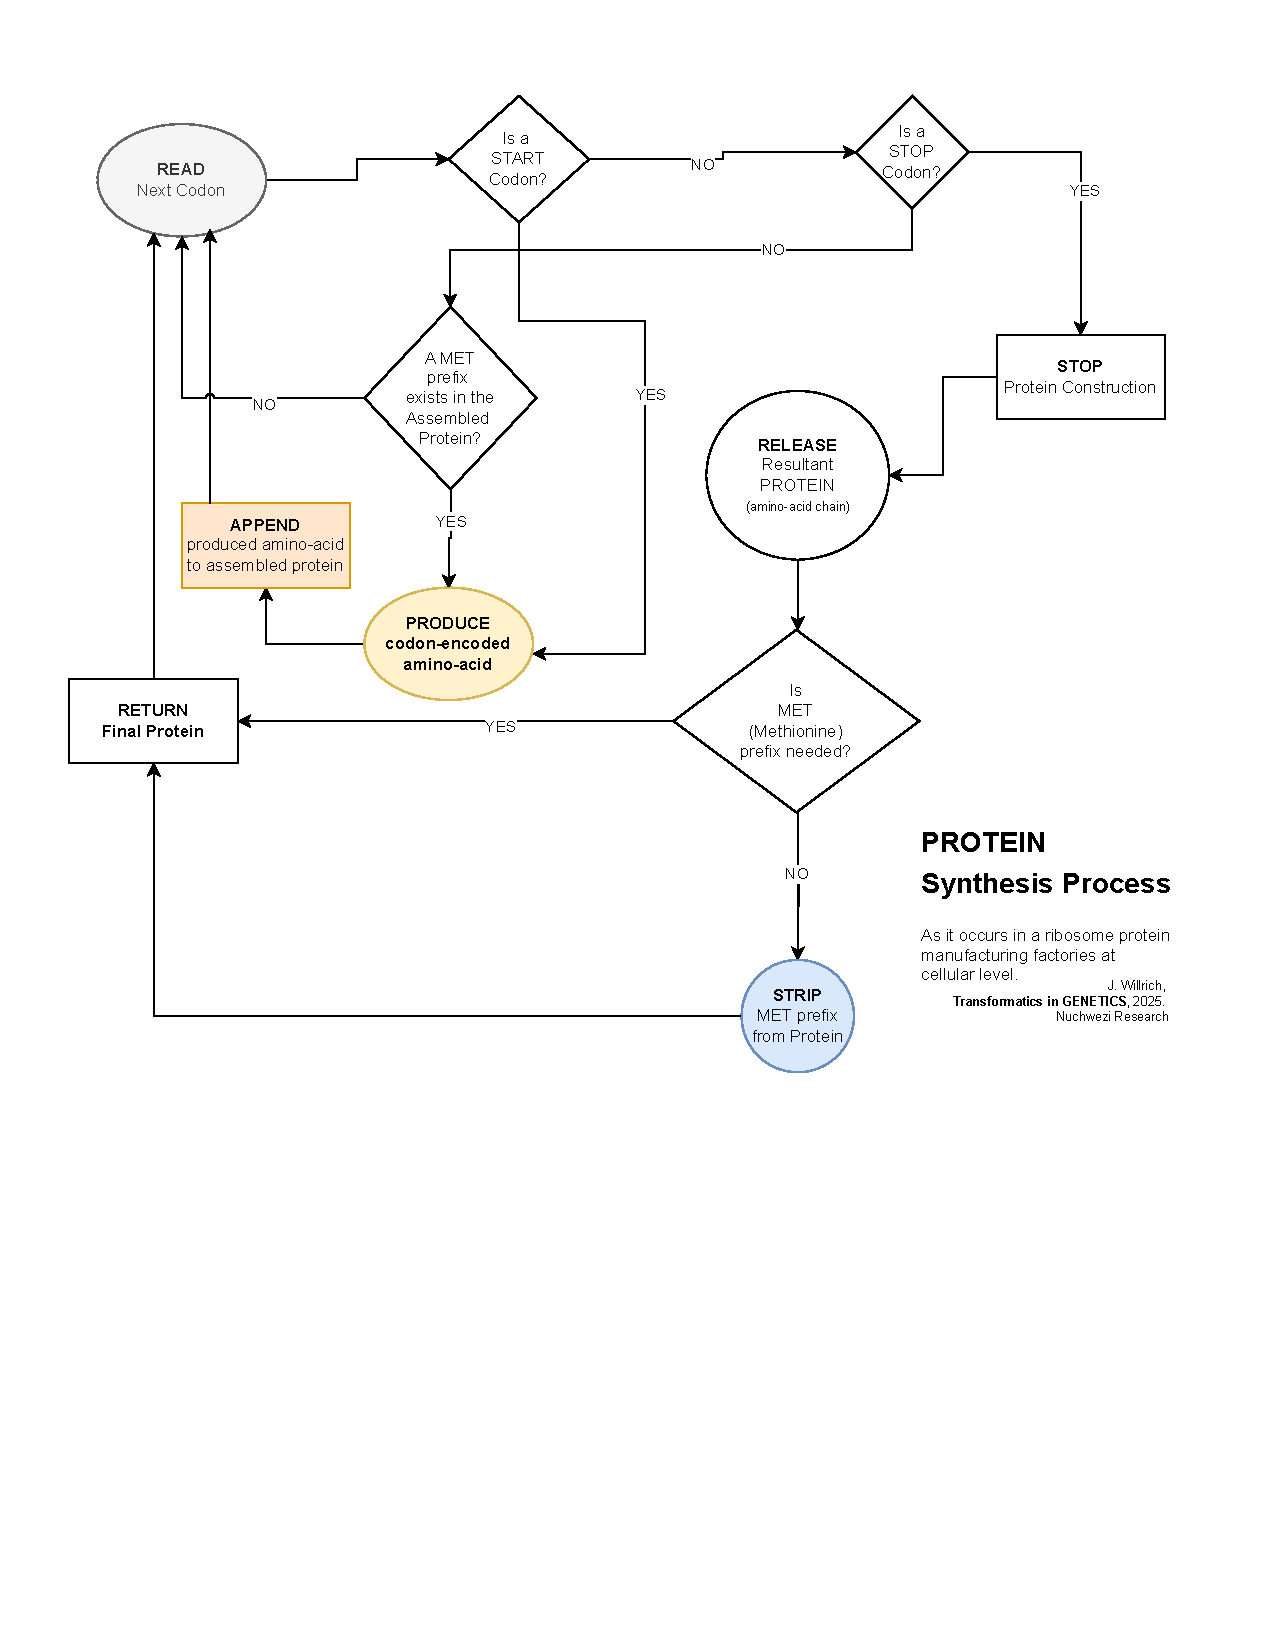
\includegraphics[trim=0cm 8cm 0cm 0cm, clip, width=0.9\textwidth,]{resources/pdfs/ProteinSynthesisProcessFlowChart.pdf}\\
   \caption{\textbf{Flow-Chart summarizing the Ribosome-based Protein-Synthesis Process in a Living Cell}}
  \label{FIG3}
  \end{center}
\end{figure}

That process which is depicted in \textbf{Figure \ref{FIG3}} is how the ribosome protein-manufacturing factory operates at a cellular level as depicted using a \textbf{Flow Chart Diagram} --- meaning, the states of the operating environment as well as those of the operator (the ribosome) are interlaced with decision-making scenarios so as to bring to mind the logic behind how the process proceeds. However, in a different diagram --- the \textbf{Ribosome State Machine} as depicted in \textbf{Figure \ref{FIG4}}, we clearly abstract everything else away and focus on what actually happens from the point-of-view of the gene code sequence processor --- the ribosome. In a way, that state machine not only depicts the various states the ribosome shall be in while operating on incoming gene-code sequences (kind of \textit{requests for solutions/solution-instances/proteins} to problems/specifications/genes) and then how it goes about producing the out-going amino-acid sequences (the proteins). It might even start to feel like the ribosome is a kind of 3D-printer, which, when presented with the specifications of a particular 3D-sequence, knows to process it (translate it) and then produce the required/specified object that is in the context of biological systems we are looking at here, essentially proteins\footnote{Of course, for someone with a background in computer science and who also has interest in designing not just computer programs but also new kinds of computers - abstract machines or not, studying the ribosome from a computing theory and computer architecture perspective --- such as so one appreciates what Instruction Set the ribosome employs; how the ribosome compares to say a Von-Neumann architecture machine; is it Turing Complete or not? How might a pure-text processing languages such as TEA\cite{lutalo2024software} implement a ribosome simulation in say a web-browser environment?\cite{lutalo_tea_web} or that failing, at least allow for the creation of a protein generator or even an entire organism generator as a simulation of how gene code sequences can be translated into sequences of multi-dimension objects?\cite{lutalo2025transformatic} etc.}.


\begin{figure}[H]
  \begin{center}
   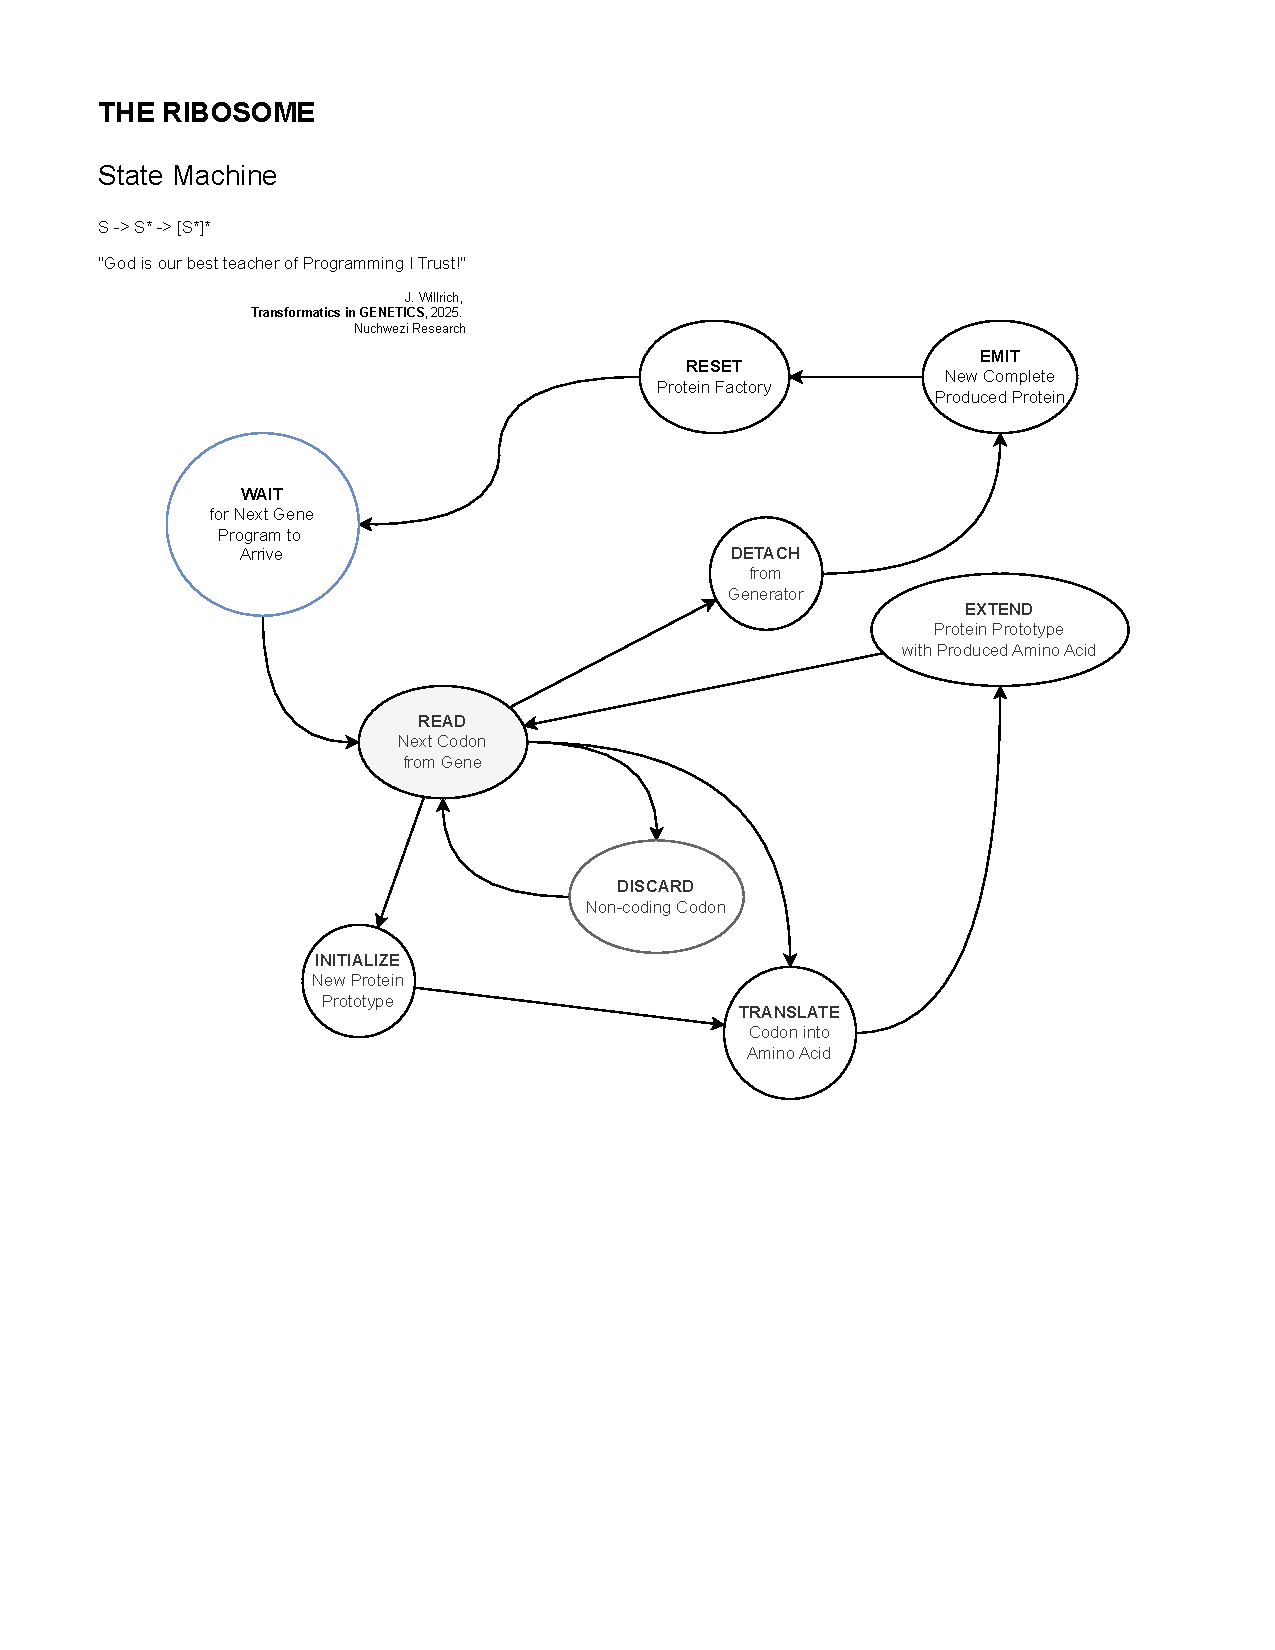
\includegraphics[trim=0cm 9cm 0cm 1.6cm, clip, width=0.9\textwidth,]{resources/pdfs/RibosomeStateMachine.pdf}\\
   \caption{\textbf{The RIBOSOME State Machine}}
  \label{FIG4}
  \end{center}
\end{figure}


Before concluding this section on biological computing systems of the sequence generator kind\cite{lutalo2025transformatic}, it should be worthwhile noting that, as depicted in \textbf{Figure \ref{FIG4}}, the process that is naturally found in every living thing's tiniest cells (excluding viruses as already saw in \textbf{Section \ref{SEC1}}, could be, as with any legitimate state machine, be used to implement a proof-of-concept ribosome processor (or a \textit{ribosome computer} --- a way to implement bio-automatons that behave like a ribosome or which process code similar to DNA and mRNA, or which generally operate on sequences to produce other (possibly more complex) sequences. Thinking of a robotic ribosome might not be something that is immediately required in contemporary medicine or in-organism computing systems, but might be a concept worth adapting or exploring for the design and implementation of self-contained robotic factories for manufacturing and outputting complex products producible via use of a sequence-processing, assembly-line kind of method just as proteins are produced in a bio-cell by the ribosome. We might for example think of ``a sequence from which a finished particular type of car can be manufactured at will" or ``a sequence from which certain kinds of sequence-form/sequence-based\footnote{Vertebrates anyone(?)} artificial and/or organic creatures or bots might be systematically produced at will or on-demand". These kinds of printers --- which, unlike just printers of things on paper, or 3D-printers that know to only produce plastic variants of models they are fed with, but which can say \textit{print a human}\footnote{Though we might touch on it in a future paper on philosophy --- e.g in \textit{Computational Mysticism}\cite{lutalo2024mysticism}, it might be interesting to air-out the author's illuminating view that unlike most other bio-mata such as beasts in the wild or fish in the seas, and definitely not as with silicon-based automatons such as GPT-powered modern \textit{disincarnate} artificial entities --- nor the likes of the ZHA qAGI\cite{jwlzha}, that the human in particular, has this peculiar attribute to them that, apart from just their material substratum as any physical robot might possess or need --- and which is say the domain of ``material producers" such as the ribosome is, and away from their conceptual/software substratum too, they seem to, or perhaps arguably, also possess a preternatural layer of existence that perhaps is or might not have anything to do with their DNA/material-blueprint. A better or more precise classification term for such [\textit{preter-}]intelligent -mata/matter(?) might be the still underground term and concept of a \textit{Psymaton} or \textbf{Psymata} --- bits of this line of discourse have been already touched on in the Psymaz Interview\cite{lutalo2025unraveling}.}, teleport a cow or a banana, etc. might be interesting to explore, as we look into the far-future, where, with humanity's ability to travel and survive in remote and/or unnatural worlds away from their biological home environments (such as Earth's biosphere), might compel them to have to develop new kinds of machines that would not only print out ideas on paper, but also complete food ready-to-eat, medicines to particular kinds of ailments, certain kinds of companion creatures or species, etc. Means to survive on/in alien worlds by leveraging smart, general sequence processors and generators. Talking of which, the next section shall help us start to appreciate this perspective of using the case of genetic code sequences and the ribosome sequence processor into the dimension of both artificial as well as conceptual or hypothetical bio-machines that like the bio-cell can produce complex things via processing of some kinds of code sequences. Bio-automata.


\section{Gene Expression in Bio-Automata Leveraging Genetic Modal Sub-Sequences (Numero-Gene Code $\rightarrow$ Ozin-Gene Code $\rightarrow$ Platonic-Form Organelles)}
\label{SEC5}

One might begin by wondering: \textbf{using the concepts from transformatics and pure mathematics, how might we model or express a general and realistic ribosome?} A plausible and meaningful solution to this problem would be to begin by acquiring or developing \textit{a rigorous and correct working definition of what a ribosome is.} The answer would follow directly from that, thus our first definition in this section; a formal definition of a ribosome in any system natural or artificial:


%\fbox{\begin{minipage}{0.9\textwidth}

\begin{defn}[A \textbf{Ribosome}]
\label{DEFRIBOSOME}
Assuming we re-write a sequence of DNA code in terms of the ordered sequence of nucleotides it contains, as in \textbf{Equation \ref{EQ3}} re-written as in \textbf{Equation \ref{EQ7}}:

 \begin{equation}
\label{EQ7}
\Theta_n = \{a_i \quad | \quad a_i = \prod\limits_{\rho \in \psi_{DNA}}^3 \rho \}:n
\end{equation}\\

$\Theta_n$ would then be any sequence of DNA-codons of length $n$, equivalent to an equivalent flat-structure ordered sequence of nucleotides of length $n \times 3$. We can then produce mRNA-codons from $\Theta_n$ as per \textbf{Transformer \ref{TRANSF1}}, so that we produce a new mRNA-codon sequence of length $n$ that is generated as such:

\begin{trans}
\label{TRANS1}
$\Theta_n \quad \xrightarrow{O_{mRNA-encode}(\cdot)} \quad \Theta^*_n;$\\
$\Theta^*_n = \{a_i^* \quad | \quad a_i^* = \prod\limits_{\rho \in \psi_{mRNA}}^3 \rho \}:n$
\end{trans}

And with $\Theta^*_n$ produced, we can then merely generate the corresponding ordered sequence of amino-acids, denoted as $[\Theta^*_n]^*$, via the following mRNA to amino-acid transformer: 

\begin{transf}[\textbf{mRNA to Amino-Acid Translator}]
\label{TRANSF2}
$\Theta^*_n \quad \xrightarrow{O_{mRNA-translate}(\cdot)} \quad [\Theta^*_n]^* \quad;$\\
\begin{enumerate}
\item $\invpi([\Theta^*_n]^*) < \invpi(\Theta^*_n)$ because we only count each codon in the source once, and as per in the rules of gene processing, all non-coding codons, stop codons and start codons (basically, codons not able to be translated into an amino-acid given the state of the gene processor --- see \textbf{Figure \ref{FIG3}} and \textbf{Figure \ref{FIG4}}) don't contribute to the generated resultant sequence in terms of sections it contains --- with the exception of the special ``Met" codon that might or might not be retained in the resultant sequence even though it is automatically included as the first produced amino-acid in any legitimate gene sequence.
\item The entire sequence $[\Theta^*_n]^*$ is a kind of 3-Dimension molecule based on the chain of amino-acids it contains, and is technically referred to as a protein.
\end{enumerate}
$\qed$
\end{transf}

A \textbf{Ribosome} then, is any combination of transformers that can result in $[\Theta^*_n]^*$ when presented with just $\Theta_n$ as per the two intermediate transformer processes \textbf{Transformer \ref{TRANSF1}} and \textbf{Transformer \ref{TRANSF2}}, and whose overall processing algorithm is as depicted in \textbf{Figure \ref{FIG3}} and its corresponding state machine as in \textbf{Figure \ref{FIG4}}. 

So, overall, a ribosome is any machine that can implement the combined transformer defined as in \textbf{Transformer \ref{TRANSF3}}:

\begin{transf}[The \textbf{Protein Generator} (A Ribosome)]
\label{TRANSF3}
$\Theta_n  \xrightarrow{O_{mRNA-encode}(\cdot)}  \Theta^*_n  \xrightarrow{O_{mRNA-translate}(\cdot)} [\Theta^*_n]^*;$\\
$\invpi([\Theta^*_n]^*) < \invpi(\Theta^*_n) = \invpi(\Theta_n) = n:$\\
$\psi_{\Theta} = \psi_{DNA} \quad \land \psi_{\Theta^*_n} = \psi_{mRNA} \quad \land \psi([\Theta^*_n]^*) = \psi_{amino-acids}$
\end{transf}

And thus, we can finally merely call any machine capable of implementing the protein generator  in \textbf{Transformer \ref{TRANSF3}} as a \textbf{Ribosome}.

\end{defn}

%\end{minipage}}
%\\


\section{Conclusion}
\label{CONC}

In this paper, we have advanced our knowledge concerning...

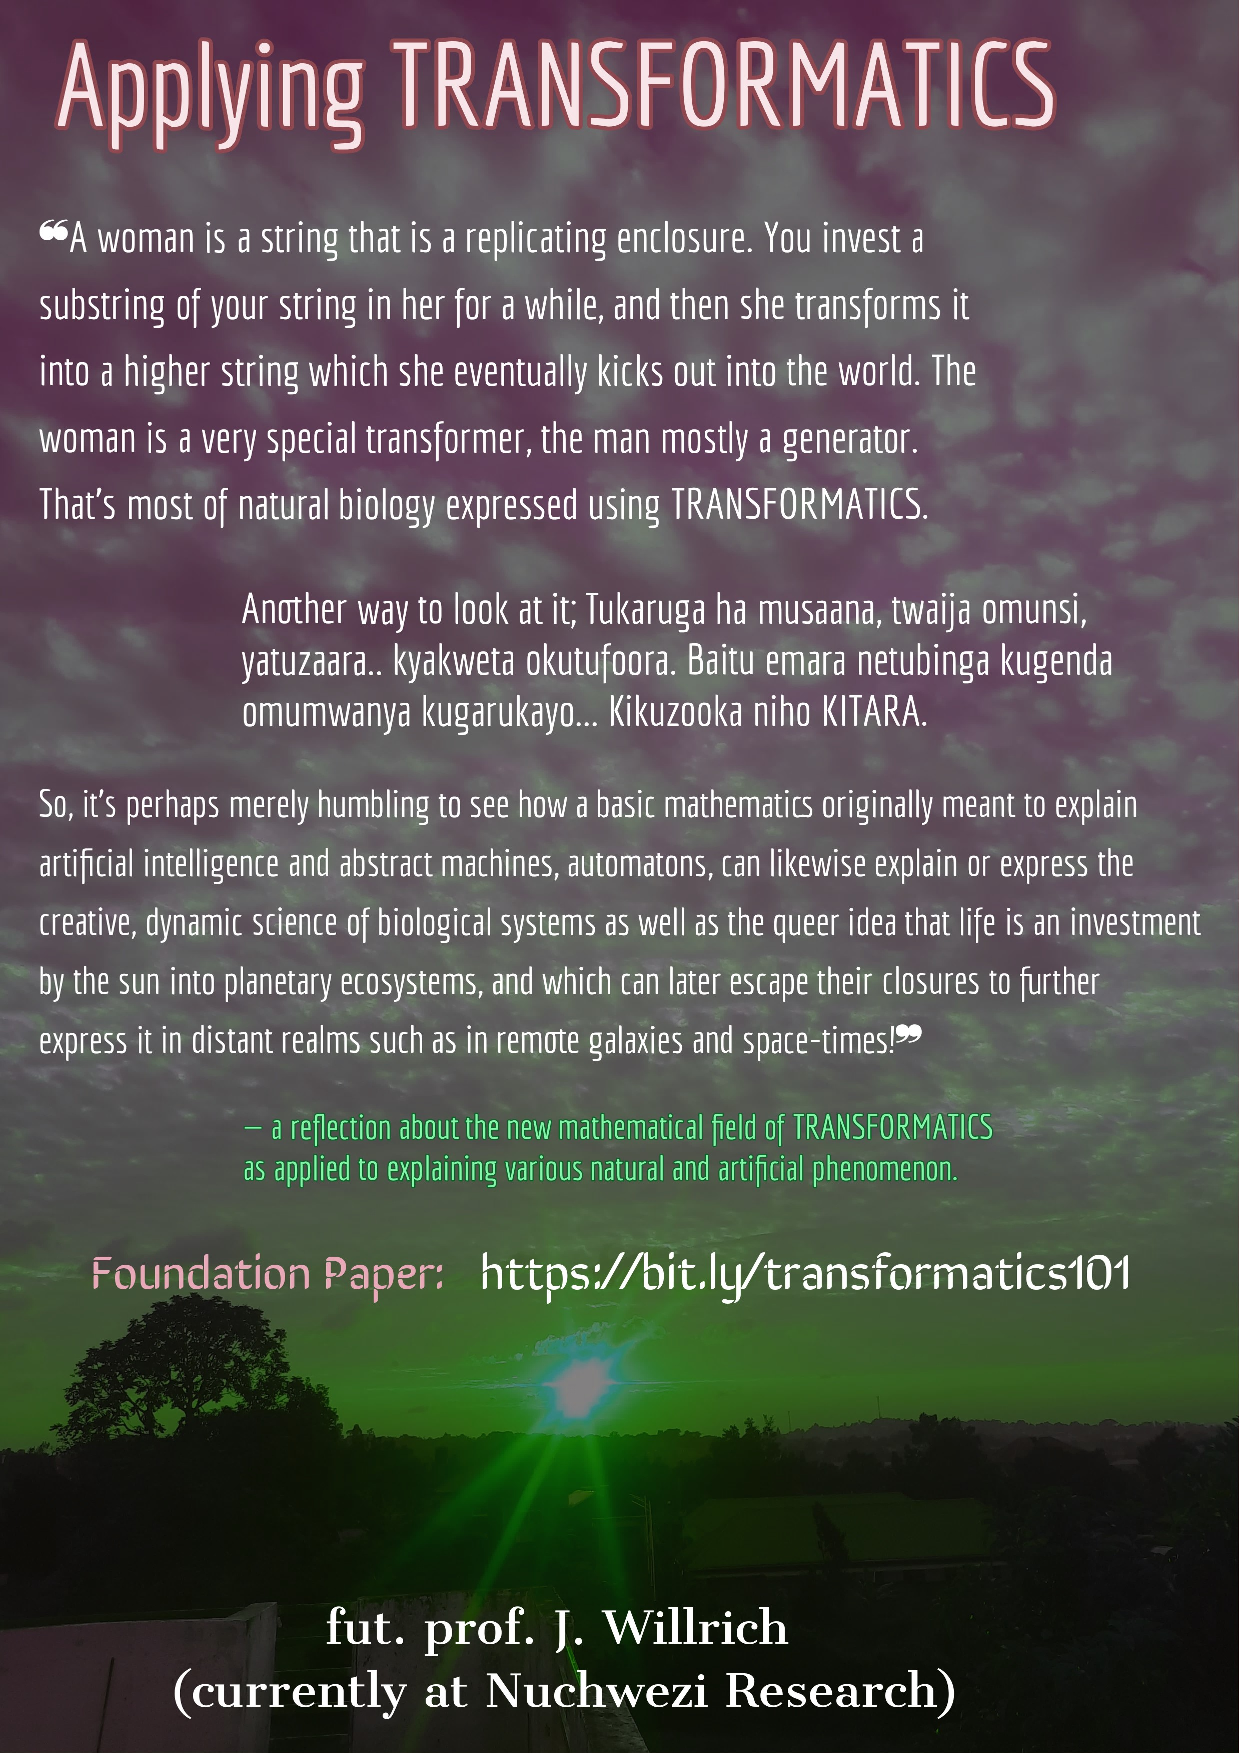
\includepdf[pages=1]{resources/pdfs/note_cover.pdf}

\bibliographystyle{unsrt}
\bibliography{references}

\comment{
\vspace{5cm}
\fbox{
\begin{minipage}{0.9\textwidth}
\textbf{TO CITE:}\\

Lutalo, Joseph Willrich (2025). \textbf{The Theory of Sequence Transformers \& their Statistics:} \textit{The 3 Information Sequence Transformer Families (Anagrammatizers, Protractors, Compressors) and 4 New and Relevant Statistical Measures Applicable to Them: Anagram Distance, Modal Sequence Statistic, Transformation Compression Ratio and Piecemeal Compression Ratio.} figshare. Online Resource. \url{https://doi.org/10.6084/m9.figshare.29505824.v3}

\end{minipage}}
\\
}


% insert [back] cover --- could just be a PNG or PDF
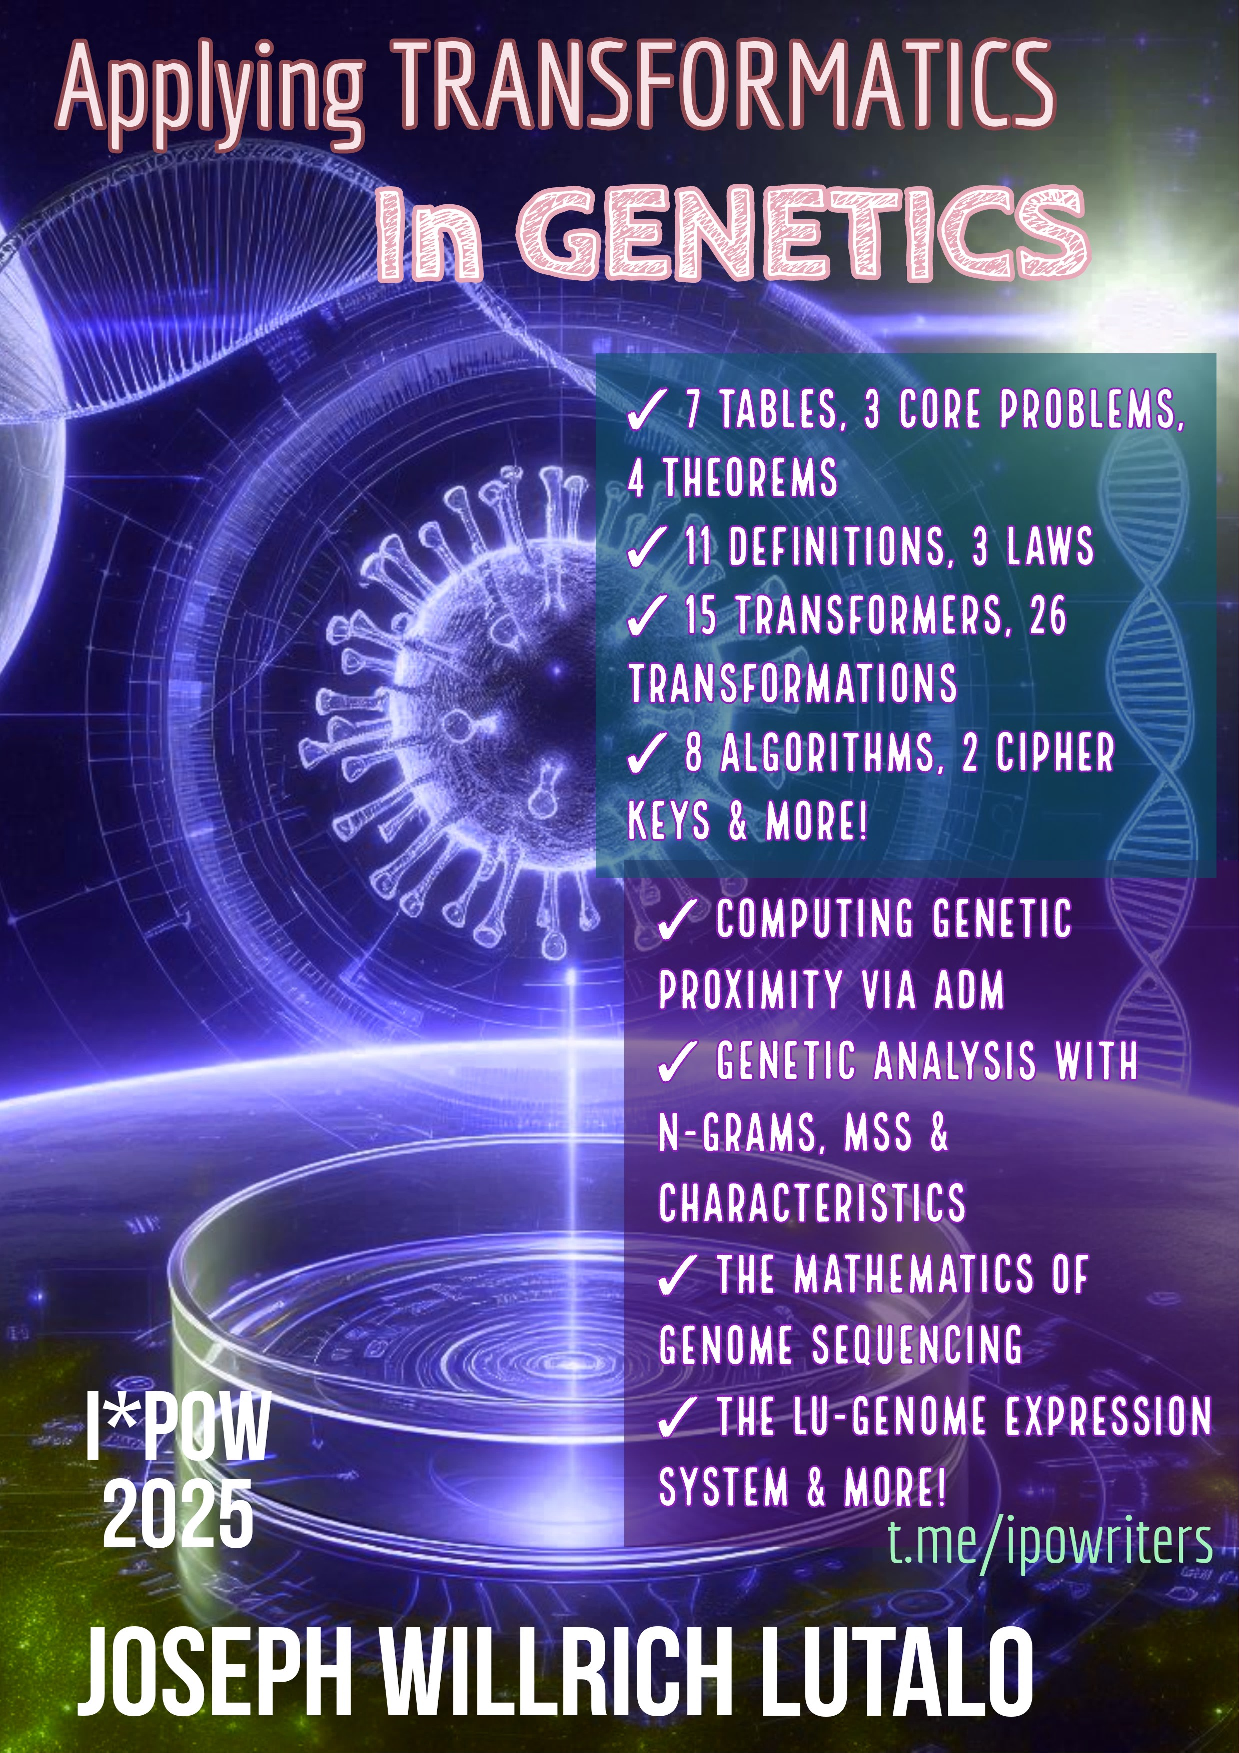
\includepdf[pages=1]{resources/pdfs/back_cover.pdf}

\end{document}